\newpage
%\pagestyle{empty}
\pagestyle{fancy}
\renewcommand{\headrulewidth}{2.4pt}
\renewcommand{\footrulewidth}{2.4pt}
\lhead{
    \setlength{\unitlength}{1mm}
    \begin{picture}(0,0)
    \put(0,0){
\includegraphics[width=0.9cm]{logo.eps}}
    \end{picture}
    }
\chead{}
\rhead{\xiaosi{合肥量子精密仪器有限公司}}
\fancyfoot[LO,RE]{\xiaosi{ASG-GT50-C用户手册}}
\cfoot{}
\fancyfoot[RO,LE]{\xiaosi\textbf{\thepage}}



\xiaoer \textbf{保证和声明}
\vspace{0.7cm}

\xiaosi \textbf{商标信息}\\
%
\includegraphics[height=2cm]{logo}
%\epsfig{figure=logo,height=2cm}
%\begin{figure}[H]
%    
\includegraphics[height=2cm]{logo}
%\end{figure}
\hspace*{0.8cm}\song{\qquad\qquad 是合肥量子精密仪器有限公司的注册商标。}
\hspace{-10.0cm}
\includegraphics[height=2cm]{logo}

\vspace{0.8cm}
\xiaosi\textbf{软件版本}
\vspace{0.4cm}

\song 软件升级可能会增加或更改产品功能, 请联系合肥量子精密仪器有限公司升级软件, 必要时我司会主动与您联系。

\vspace{0.8cm}
\xiaosi\textbf{声明}
\song
\begin{itemize}
 \item 本公司产品受中国及其他国家和地区的专利( 包括已取得和正在申请的专利)保护。
 \item 本公司拥有改变产品规格及价格的权利。
 \item 本手册提供的信息取代以往出版的任何资料。
 \item 未经我司事先书面许可, 不得影印、 复制或改变本手册的任何部分。
 \item 用户一旦使用产品, 即视为对本声明的全部内容认可和接受。
\end{itemize}

\vspace{0.6cm}
%\xiaosi\textbf{产品认证}
%\vspace{3cm}

\xiaosi\textbf{联系我们}
\song
\begin{itemize}
 \item 秦熙: 合肥量子精密仪器有限公司首席技术官
 \item 电子邮箱: sale@qpdtek.com
 \item 电话: +86 13816630636
\end{itemize}

%\noindent\song
%如果您在使用此产品或本手册的过程中有任何问题或需求,可与我司联系:\\
%\song 秦熙: 合肥量子精密仪器有限公司, 首席技术官\\
%\song 电子邮箱: sale@qpdtek.com\\
% 电话: +86 13816630636

\newpage
\xiaoer \textbf{安全要求}
\vspace{1.1cm}

\noindent\sanhao\textbf{一般安全概要}
\vspace{0.7cm}
\song

为避免可能的危险,以及防止损坏本产品和与本产品连接的任何设备,用户需了解以下安全措施,并按照规定使用本产品。

\vspace{0.7cm}
\noindent{\color{red}\textbf{使用正确的电源线}}

\vspace{0.2cm}
只允许使用我司所提供的电源线。

\vspace{0.7cm}
\noindent{\color{red}\textbf{确保供电电源正确}}

\vspace{0.2cm}
为避免对操作人员造成伤害或损坏产品,请在使用产品前仔细阅读本手册,并确保产品供电电源正确。

\vspace{0.7cm}
\noindent{\color{red}\textbf{请勿开盖操作}}

\vspace{0.2cm}
请勿在产品机箱打开时运行本产品。

\vspace{0.7cm}
\noindent{\color{red}\textbf{避免电路外露}}

\vspace{0.2cm}
若机箱内电路板元件有外露, 请勿触碰并立即与我司联系。

\vspace{0.7cm}
\noindent{\color{red}\textbf{保持良好的散热条件}}

\vspace{0.2cm}
为避免因机箱内电路板过热而损坏仪器,在使用本产品的过程中请勿堵住通风口。

\vspace{0.7cm}
\noindent{\color{red}\textbf{请勿在潮湿环境下操作仪器}}

\vspace{0.2cm}
为避免产品内部电路出现短路等危险情况, 请勿在潮湿环境下操作仪器。


\vspace{0.7cm}
\noindent{\color{red}\textbf{请勿靠近易燃易爆物品}}

\vspace{0.2cm}
为避免人身伤害或产品损坏, 严禁易燃易爆物靠近本产品。

\vspace{0.7cm}
\noindent{\color{red}\textbf{注意搬运安全}}

\vspace{0.2cm}
为避免对产品面板上的按键、 接口、 指示灯等部件造成损坏, 请注意搬运安全。

\vspace{0.7cm}
\noindent{\color{red}\textbf{远离高温环境}}

\vspace{0.2cm}
为避免发生危险,严禁将本产品放置于高温环境中。

\newpage
\vspace{0.7cm}
\noindent{\color{red}\textbf{严禁不具备操作能力的人使用本产品}}

\vspace{0.2cm}
为避免造成人身伤害或产品损坏,严禁不具备操作能力的人( 如老人、 儿童)使用本产品。

\vspace{0.7cm}
\noindent{\color{red}\textbf{保养与清洁}}

\vspace{0.2cm}
请经常对产品进行清洁, 方法如下: 先断开电源, 再用干抹布轻轻擦拭产品机箱外部。

%\vspace{0.6cm}
%\noindent{\color{red}\textbf{怀疑产品出故障时, 请立即联系我司}}
%
%如果您怀疑本产品出现故障, 请联络我司授权的维修人员进行检测。 任何由未经我司允许的维护、 调整或零件更换而造成损失, 我司不承担任何责任。

\newpage
%\pagestyle{plain}
%\setcounter{page}{1}
\noindent\huge \textbf{ASG-GT50-C} \xiaoer\textbf{任意序列发生器简介}
\vspace{0.6cm}

\normalsize ASG-GT50-C\song 系列是我司研发的高性能方波/延时发生器,又称任意序列发生器。该任意序列发生器拥有8个相互独立的方波输出通道。如图1所示,该任意序列发生器可以连续输出高电平最短7.5 ns,最长达2.6 s,低电平最短10 ns,最长达2.6 s 宽度的方波,且连续可调,同时每个方波上升沿和下降沿的时间分辨率可达50 ps。
\begin{figure}[ht]
\centering
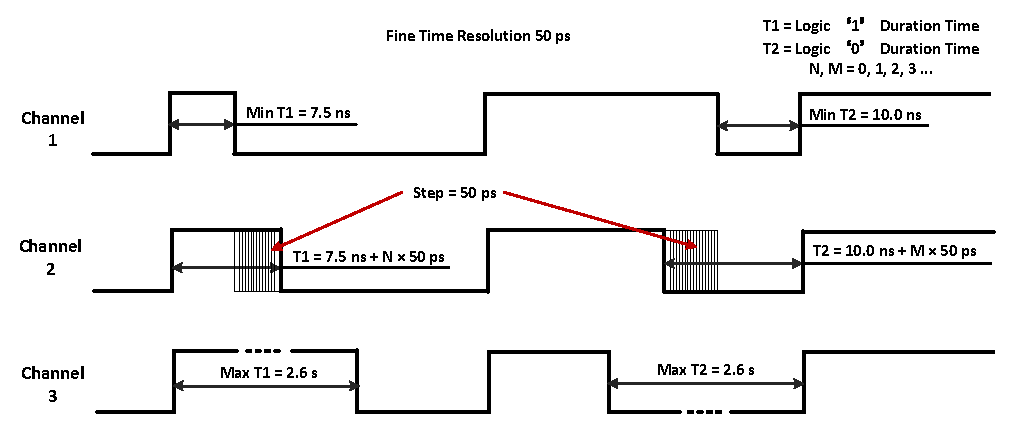
\includegraphics[width=14.5cm,height=6cm]{fig_shixu}
\caption{方波时序图}\label{fig:fig1}
\end{figure}
\vspace{0.5cm}

\makeatletter
\def\hlinewd#1{%
  \noalign{\ifnum0=`}\fi\hrule \@height #1 \futurelet
   \reserved@a\@xhline}
\makeatother
%\newcommand\vlinewd#1{\vrule width #1}
\definecolor{myblue}{rgb}{.46,.42,.80}
\definecolor{tabcolor_top}{rgb}{255,255,255}
\definecolor{tabcolor}{rgb}{255,255,255}
\noindent\sanhao\textbf{产品主要特征}
\vspace{0.2cm}
\song
\begin{table}[H]
\normalsize
\rowcolors{2}{gray!20}{gray!20}
\begin{tabular}{m{13.5cm}}
\rowcolor{gray!20}
\arrayrulecolor{tabcolor_top}\toprule[1.8pt]
方波/序列输出时间精度:50 ps\\\arrayrulecolor{tabcolor}\midrule[1.2pt]
独立方波/序列输出通道数:8个 \\\arrayrulecolor{tabcolor}\midrule[1.2pt]
单脉冲动态范围为7.5 ns至2.6 s\\\arrayrulecolor{tabcolor}\midrule[1.2pt]
高长期稳定度:脉冲宽度 < 500 ms 时,抖动 < 25 ps \\\arrayrulecolor{tabcolor}\midrule[1.2pt]
方波序列的存储内存可达4 GB\\\arrayrulecolor{tabcolor}\midrule[1.2pt]
采用USB接口通信\\\arrayrulecolor{tabcolor}\midrule[1.2pt]
配备方波序列编辑软件\\
\arrayrulecolor{tabcolor_top}\bottomrule[1.8pt]
\end{tabular}
\end{table}

%\begin{itemize}
% \item 50 ps时间分辨率的方波输出。
% \item 8个通道独立自定义方波输出。
% \item 单脉冲动态范围为5 ns至2.6 s,且无死时间。
% \item 高长期稳定度。
% \item 集成了高速计数读出功能。
% \item 方波序列的存储内存可以达到4 GB。
% \item 采用USB接口通信。
% \item 配备方波序列编辑软件。
%\end{itemize}

%\vspace{0.5cm}
%\newpage
\noindent\sanhao\textbf{产品技术规格参数}
\vspace{0.5cm}

\noindent\xiaosi\textbf{外观特征:}
\vspace{0.1cm}
\song
\begin{table}[H]
\normalsize
\rowcolors{2}{gray!20}{gray!20}
\begin{tabular}{m{6.5cm}|m{6.5cm}}
\rowcolor{myblue}
%\arrayrulecolor{tabcolor_top}\toprule[1.8pt]
\color{white}参数名称& \color{white}参数值\\\arrayrulecolor{tabcolor}\midrule[1.2pt]
机身材质& 铝合金外壳\\\arrayrulecolor{tabcolor}\midrule[1.2pt]
机身颜色& 银灰色\\\arrayrulecolor{tabcolor}\midrule[1.2pt]
产品尺寸& 207*122*65 mm\\
%\arrayrulecolor{tabcolor_top}\bottomrule[1.8pt]
\end{tabular}
\end{table}

%\begin{itemize}
 %\item 机身材质: 铝合金外壳
 %\item 机身颜色: 银灰色
 %\item 产品尺寸: 207*122*65 mm
%\end{itemize}

\vspace{0.4cm}
%\newpage
\noindent\xiaosi\textbf{电气特性:}
\vspace{0.1cm}
\song
\begin{table}[H]
\normalsize
\rowcolors{2}{gray!20}{gray!20}
\begin{tabular}{m{6.5cm}|m{6.5cm}}
\rowcolor{myblue}
%\arrayrulecolor{tabcolor_top}\toprule[1.8pt]
\color{white}参数名称& \color{white}参数值\\\arrayrulecolor{tabcolor}\midrule[1.2pt]
工作电压& DC 12 V\\\arrayrulecolor{tabcolor}\midrule[1.2pt]
待机电流& 约0.85 A\\\arrayrulecolor{tabcolor}\midrule[1.2pt]
工作电流& ≤ 1.2 A\\\arrayrulecolor{tabcolor}\midrule[1.2pt]
最大功率& 约12 W\\
%\arrayrulecolor{tabcolor_top}\bottomrule[1.8pt]
\end{tabular}
\end{table}

%\begin{itemize}
% \item 工作电压: DC 12 V
% \item 待机电流: 约 0.85 A
%\item 工作电流: ≤1.2 A
 %\item 最大功率: 约 12 W
%\end{itemize}

\vspace{0.4cm}
\noindent\xiaosi\textbf{技术参数:}
\vspace{0.1cm}
%\song
\begin{table}[H]
%\Large
\rowcolors{2}{gray!20}{gray!20}
\begin{tabular}{m{6.5cm}|m{6.5cm}}
\rowcolor{myblue}
%\arrayrulecolor{tabcolor_top}\toprule[1.8pt]
\color{white}参数名称& \color{white}参数值\\\arrayrulecolor{tabcolor}\midrule[1.2pt]
时间分辨率& 50 ps\\\arrayrulecolor{tabcolor}\midrule[1.2pt]
最小脉冲宽度& 7.5 ns \\\arrayrulecolor{tabcolor}\midrule[1.2pt]
最大脉冲宽度& 2.6 s\\\arrayrulecolor{tabcolor}\midrule[1.2pt]
最大方波输出通道数& 8个\\\arrayrulecolor{tabcolor}\midrule[1.2pt]
方波序列存储内存& 4 GB\\\arrayrulecolor{tabcolor}\midrule[1.2pt]
单通道最多输出方波个数&  4×$10^{7}$个\\\midrule[1.2pt]
耦合方式& DC 50 ohm\\\arrayrulecolor{tabcolor}\midrule[1.2pt]
输出低电平& 0 V\\\arrayrulecolor{tabcolor}\midrule[1.2pt]
输出高电平& 3.3 V\\\arrayrulecolor{tabcolor}\midrule[1.2pt]
%\arrayrulecolor{tabcolor_top}\bottomrule[1.8pt]
\end{tabular}
\end{table}


%\begin{itemize}
% \item  时间分辨率: 50 ps
% \item 最小脉冲宽度: 5 ns
% \item 最大脉冲宽度: 2.6 s
% \item 最大方波输出通道数: 8
% \item  方波序列存储内存: 4 GB
%\item  单通道最多输出方波个数: $4\times 10^8$个
% \item  耦合方式: DC 50 ohm
% \item  输出低电平: 0 V
% \item  输出高电平: 3.3 V
% \item  输入低电平: -5.2 V 至 +0.4 V
% \item  输入高电平: +0.6 V 至 +3.5 V
% \item  最大计数率: 50 MHz
% \item  单个计数使能信号脉冲宽度范围: 5 ns 至 5000 s
%\end{itemize}

\vspace{0.4cm}
%\newpage
\noindent\sanhao\textbf{产品应用}
\vspace{0.3cm}
\song
\begin{table}[H]
%\Large
\rowcolors{2}{gray!20}{gray!20}
\begin{tabular}{m{13.5cm}}
\rowcolor{gray!20}
\arrayrulecolor{tabcolor_top}\toprule[1.8pt]
高时间精度的脉冲/序列发生器\\\arrayrulecolor{tabcolor}\midrule[1.2pt]
高精度同步信号发生器 \\\arrayrulecolor{tabcolor}\midrule[1.2pt]
延时发生器\\\arrayrulecolor{tabcolor}\midrule[1.2pt]
\arrayrulecolor{tabcolor_top}\bottomrule[1.8pt]
\end{tabular}
\end{table}

\newpage
\qquad

%\begin{itemize}
 %\item 高时间精度的脉冲/序列发生器
 %\item 延时发生器
 %\item 高精度计时器
 %\item 高精度同步器
 %\item 高速计数读出
%\end{itemize}
